\documentclass{article}


% if you need to pass options to natbib, use, e.g.:
%     \PassOptionsToPackage{numbers, compress}{natbib}
% before loading neurips_2023

% ready for submission
\usepackage[final]{neurips_2023}

% to avoid loading the natbib package, add option nonatbib:
%    \usepackage[nonatbib]{neurips_2023}


\usepackage[utf8]{inputenc} % allow utf-8 input
\usepackage[T1]{fontenc}    % use 8-bit T1 fonts
\usepackage{hyperref}       % hyperlinks
\usepackage{url}            % simple URL typesetting
\usepackage{booktabs}       % professional-quality tables
\usepackage{amsfonts}       % blackboard math symbols
\usepackage{nicefrac}       % compact symbols for 1/2, etc.
\usepackage{microtype}      % microtypography
\usepackage{xcolor}         % colors
\usepackage{graphicx}       % addtional package for show figures


\begin{document}


\maketitle


%%%%%%%Part 3 Audio Features Start%%%%%%%%%

\section{Audio Features}   

\subsubsection{(a) Feature selection \& down‑projection}  % third‑level
We inspected the 13 frame keys provided in each \texttt{.npz} file and removed
strongly correlated or low‑value duplicates (\texttt{power}$\approx$\texttt{energy}, 
\texttt{mfcc\_delta2}, \texttt{flatness}).  
The nine retained groups are listed in Table~\ref{tab:feat}.  
A StandardScaler followed by PCA keeps \textbf{95.4\,\%} variance in 62
components (Figure~\ref{fig:pca}); a second PCA reduces the dimension to~50.

\begin{table}[h]
	\caption{Retained frame feature groups (total $140$\,dims).}
	\label{tab:feat}
	\centering
	\begin{tabular}{lcl}
		\toprule
		Group & \#dims & Reason \\ \midrule
		Mel spectrogram            & 64 & dense spectral envelope \\
		MFCC + $\Delta$            & 64 & static \& dynamic timbre \\
		Spectral contrast          & 7  & noise vs.\ harmonic      \\
		Centroid, bandwidth, flux  & 3  & brightness / variation   \\
		Energy, ZCR                & 2  & loudness / noisiness     \\ \bottomrule
	\end{tabular}
\end{table}

\begin{figure}[h]
	\centering
	% PCA cumulative variance plot
	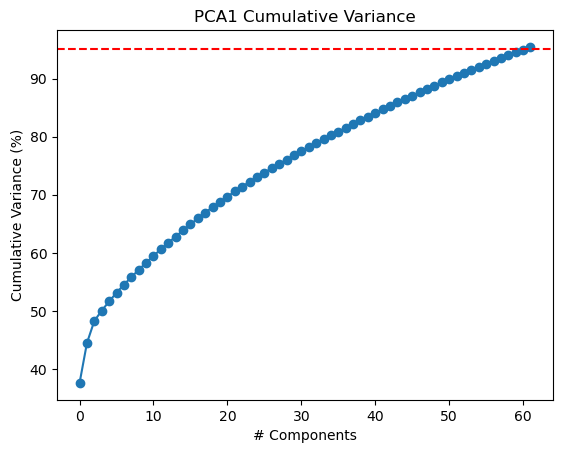
\includegraphics[width=.55\linewidth]{figs_tang/03_pca_cumulative_variance.png}
	\caption{Cumulative explained variance of PCA$_1$ 
		(\textcolor{red}{dashed}=95\%).}
	\label{fig:pca}
\end{figure}

\subsubsection{(b) Fixed‑length region vectors}
Each annotated interval $(t_\mathrm{on},t_\mathrm{off})$ and its silent
counterpart is mapped to a 50‑D vector by averaging the projected frame
vectors:
\[
\mathbf v = \frac1N \sum_{t=i_0}^{i_1-1}
\mathrm{PCA}_2\bigl(\mathrm{PCA}_1(\mathrm{Scaler}(\mathbf f_t))\bigr).
\]
The procedure produces \textbf{51\,966} region vectors 
(\,35\,723 events; 16\,243 silence).

\subsubsection{(c) Clustering \& silence analysis}
A $k$‑Means sweep ($k=4\dots30$) yields the highest silhouette 
($0.18$) for $k=4$ (Figure~\ref{fig:elbow}).  
Cluster composition is summarised in Table~\ref{tab:cluster}; 
cluster~\#2 aggregates \textbf{84\,\%} of all silence vectors, while the
remaining silence mainly lives in cluster~\#3.

\begin{figure}[h]
	\centering
	%Elbow+Silhouette plot
	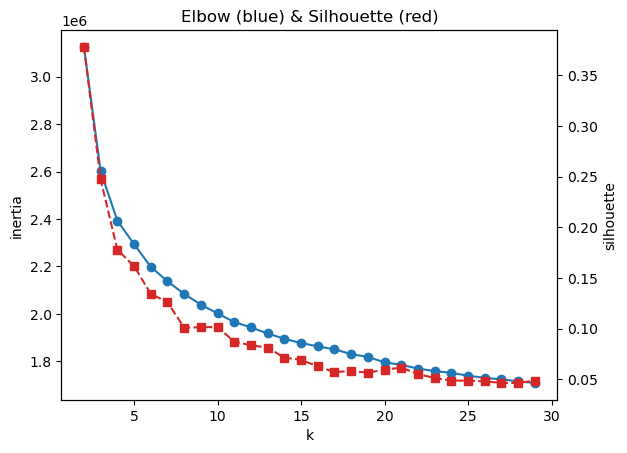
\includegraphics[width=.55\linewidth]{figs_tang/03_elbow_silhouette.png}
	\caption{Elbow (blue) and silhouette (red) curves for $k=4\dots30$.}
	\label{fig:elbow}
\end{figure}

\begin{table}[h]
	\caption{Cluster statistics for $k=4$.}
	\label{tab:cluster}
	\centering
	\begin{tabular}{cccc}
		\toprule
		id & size & silence (\%) & perceptual label \\ \midrule
		0 & 17\,944 & 19 & vehicle\,/\,rumble \\
		1 & 15\,745 & 11 & sharp metallic hits \\
		\textbf{2} & 6\,447 & \textbf{84} & near‑silence \\
		3 & 11\,830 & 47 & diffuse ambience \\ \bottomrule
	\end{tabular}
\end{table}

Figure~\ref{fig:pca_scatter} visualises the clusters in PCA‑2D and highlights
the concentrated silence cloud.

\begin{figure}[h]
	\centering
	% PCA scatter plots
	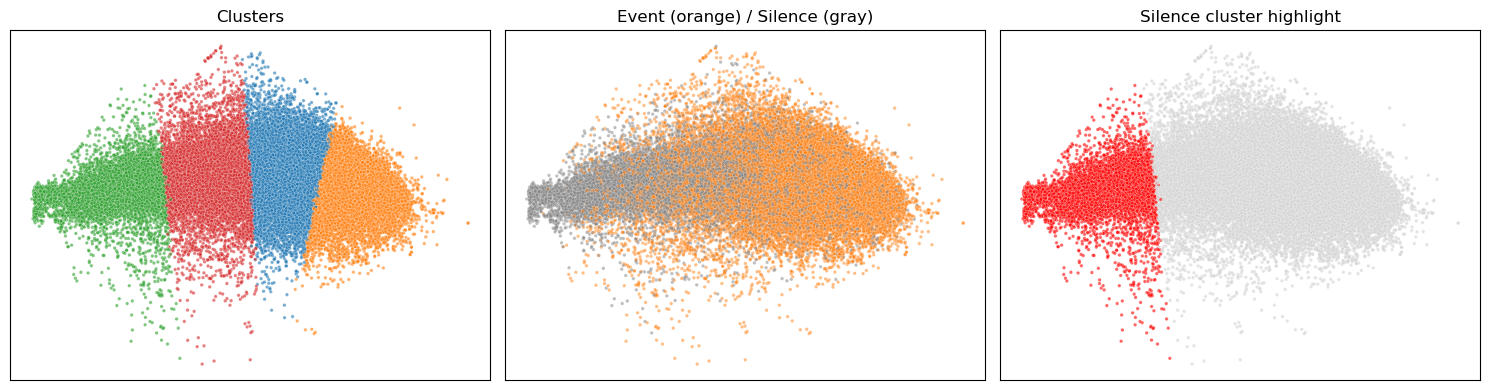
\includegraphics[width=.45\linewidth]{figs_tang/03_pca_clusters.png}
	\caption{Left: clusters in PCA‑2D; Right: event (orange) vs.\ silence (grey).}
	\label{fig:pca_scatter}
\end{figure}

These four clusters already separate silence and three broad acoustic families,
providing useful pseudo‑labels for downstream detector training.

%%%%%%%Part 3 Audio Features Finish%%%%%%%%%


\end{document}